\chapter{Monte Carlo Methods Applied to the Ising Model}

A short review of the Monte Carlo (MC) methods used to solve the Ising Model in the current paradigm is presented. There will be a focus on the famous Metropolis Method and the Wang-Landau sampling. 

\section{Metropolis Method}

The classic Metropolis method, introduced in 1953 by Metropolis et al. \cite{Metropolis1953}, belongs to the Markov chain Monte Carlo (MCMC) class of algorithms. These algorithms exploit the fact that if we construct a Markov chain that has a specific equilibrium distribution one can obtain samples recording the states generated by the Markov chain. 

In a brief fashion, a Markov chain is a stochastic model that describes a sequence of possible events, in this case microstates,in which the probability of transiting to another state depends on the current state. This way the probability of the next state, $S_j$, given the current state, $S_i$, can be written as 
\begin{equation}
	P(S_j, t) = \sum_i W(S_i \rightarrow S_j) P(S_i, t),
\end{equation}
where $W(S_i \rightarrow S_j) \equiv W_{ij}$ is the transition probability to move from the state $i$ to $j$. We require that 
\begin{equation}
	W_{ij}  \geq 0 \quad \quad \quad \quad \quad \sum_j W_{ij}=1.
\end{equation}
The master equation considers the change of the probability of the next state with time, $t$,
\begin{equation}
	\frac{dP(S_j, t)}{dt} = \sum_i \left[ W_{ij}P(S_i, t) - W_{ji} P(S_j,t)  \right].
\end{equation}
In the equilibrium regime, the master equation has to equal $0$, and we get the detailed balance condition for the equilibrium probability $P_{eq}(S_j)$,
\begin{equation}
	W_{ji}P_{eq}(S_j) = W_{ij}P_{eq}(S_i).
\end{equation}

The objective of Metropolis sampling is to generate canonical configurations with an equilibrium probability
\begin{equation} \label{eq:met_prob_eq}
	P_{eq}(E_i) = \frac{\exp(-\beta E_i)}{Z}.
\end{equation}
Here $Z$ is the partition function, however this is usually not know before hand. When considering a Markovian process we generate each new configuration from the preceding one avoiding this problem. As a result the difference of energy between the two states is needed, $\Delta E = E_i - E_j$ and the transition probability of given as

\begin{equation}
	W_{ij} = \twopartdef { \tau_0^{-1} \exp(-\beta \Delta E) } {\Delta E \geq 0} {\tau_0^{-1}} {\Delta E < 0}
\end{equation}
where $\tau_0^{-1}$ is the time required to attempt a spin-flip.  We often set this time unit to one.

This way the Metropolis method applied to the Ising Model \cite{Landau_Book}, with a fixed external magnetic field and a fixed temperature, goes as follows:

\begin{enumerate}
\item Choose an initial state;
\item Choose a spin $i$ and perform a spin-flip;                                                                                                                                       
\item Calculate the energy change from that spin-flip, $\Delta E$;
\item Accept the flip with a probability $\min \left( 1, \exp(-\beta \Delta E) \right)$; 
\item When the system reaches equilibrium, measure any thermodynamic quantity needed;                                                                                                        
\item Go back to (2) and repeat until there is enough samples of the thermodynamic variables.                                                                                                                    
\end{enumerate}
Note that we accept the spin flip if a given uniformly random number $r, r \in [0,1]$, is less or equal to the acceptance criteria. Typically in Monte Carlo simulations we define the MC time as the amount of trial flips equal to the number of spins in our lattice, N.

\subsection{Success and Limitations}

The Metropolis sampling proposed by Metropolis et al. \cite{Metropolis1953}, can be successfully applied to an array of models, ranging from widely studied quantum ensembles and gases simulations to state-of-the-art protein and peptide simulations and to machine learning and neural networks. The following paragraphs will be directed to magnetic systems, like the Ising model, but they can be extrapolated to others physical systems. 

When estimating thermodynamic variables the simulation must reach the equilibrium stage, where the probability distribution takes the form of Equation \ref{eq:met_prob_eq}. Then we take a measurement at  each MC time, resulting in $R$ total values for that variable. At the end the average of that variable, $A$, is taken $\langle A \rangle = \frac{1}{R} \sum_i A_i$. 
For large systems the time taken to reach equilibrium stage is often very long thus making the simulation time consuming. 
This is worsened by the fact that to study how some thermodynamic variable $A$ changes over a wide range of temperatures or applied fields intensities, we need to run multiple Metropolis simulations for each temperature and field intensity values, making this process very time-consuming.

Lastly there is another shortcoming known as critical slowing down. In short, for computations where the temperature is near the critical temperature, $T_C$, the sampling slows down, meaning that it is more time-consuming for the computations to reach the equilibrium stage, thus slowing down the overall simulation \cite{Landau_Book}.

\section{Wang-Landau Sampling}

Since its introduction, the Metropolis sampling was the go-to method to study phase transitions and critical phenomena in condensed matter physics and statistical mechanics. In the final decades of the 20th century scientists were committed to develop new methods that could overcome the shortcomings of the Metropolis sampling. Various methods were proposed such as the cluster flip algorithms, where Swendsen and Wang where pioneers, and the multicanonical ensemble method \cite{WL_Original}. The first solved the critical slowing down present in the Metropolis and the second could sample rough energy landscapes with ease. 

In 2001, Fugao Wang and David P. Landau \cite{WL_Original, WL_Edu} proposed a new Monte Carlo method, now called the Wang-Landau (WL) method or sampling. The goal of this method diverges from the goal of previous methods. Instead of generating configurations with a canonical probability, this method tries to estimate the canonical partition function
\begin{equation}
	Z = \sum_E g(E) \exp(-\beta E),
\end{equation}
through the estimation of the density of states $g(E)$ from a flat histogram in the phase space.

The main difficulty of a simple random walk in the energy space is that the walker would spend most of its time in the highest probable states thus making the random walk ineffective. The idea of the Wang-Landau sampling is to do a random walk,Metropolis like, and accepting the new states with a probability proportional to the inverse to their DoS $\frac{1}{g(E)}$. Doing this we obtain a flat histogram meaning that each macrostate has the same probability of being visited.  
Since $g(E)$ is unknown \textit{à priori}, in each step of the random walk, $g(E)$ is also being constructed.

The proposed algorithm computed the DoS but, it can also estimate the JDoS by performing the random walk in the phase space composed by energy, $E$, and the second order parameter, in our case, the magnetization of the system, $M$. This comes with a downside, since the JDoS has much more information than the DoS it takes much longer compute.
Later in 2006, Landau et al. \cite{WL_Cont}, presented a modification of the WL called the global updates method. This is a much harder version to implement but is much more efficient when sampling 2D discrete phase spaces and continuous phase spaces \cite{Poulain2006}.  

\subsection{Algorithm}

First we start with an arbitrary configuration of spins and a guess for the density of states. Usually,this  guess is $g(E, M)=1$. Choosing a random site in our lattice, we perform a trial flip and compute the energy-magnetization pair before the trial, $(E_i, M_i)$, and after, $(E_j,M_j)$. The new configuration is accepted with a probability
\begin{equation}
	P((E_i, M_i) \rightarrow (E_j, M_j)) = \min\left(1, \frac{g(E_i, M_i)}{g(E_j, M_j)}\right).
\end{equation}
Whether the configuration is accepted or rejected, we have to update the histogram and refine the DoS estimation. This way, being the system in the state $(E, M)$,
\begin{equation*}
	H(E, M) = H(E,M)+1,
\end{equation*}
and we multiply the current value of the DoS by a modification factor, $f > 1$,
\begin{equation*}
	g(E,M)=f \times g(E,M).
\end{equation*}
A reasonable choice for the initial value of the modification factor if $f_0 = e$. If $f_0$ is too small, the simulation will take a very long time to reach all of the possible macrostates, $(E,M)$. If it is too large, then we will have large statistical errors.  
This process is repeated until the histogram is considered "flat", all of the possible energies have been visited the same number of times. As it is impossible to obtain a $100\%$ flat histogram, we define a rule for flatness as $\min(H(E, M)) > \langle H(E, M) \rangle \times p$; $p$ is chosen according to the size of the problem. For small cases, such as the two dimensional Ising model, $p$ can be set as high as $0.95$, but for larger systems the flatness condition may never be satisfied if $p$ is near unity.  
Once a flat histogram is reached, we set $H(E, M)=0$, keep the estimation of the DoS and reduce the modification factor, $\sqrt{f_{i}} \rightarrow f_{i+1}$ and continue the random walk. We stop the simulation if $f<f_{final}$, where $f_{final}$ is a number very close to one (often $f_{final} \sim 1+1E-8$). 

At the end, the method gives us the relative density of states. To determine the normalized DoS we can use the fact that 
\begin{equation}
	\sum_{E,M} g(E,M) = 2^N.
\end{equation}
We can also use number of configurations that have a designated magnetization $\Omega(M)$ to normalize the JDoS. This way we normalize the JDoS in a sequential manner magnetization through magnetization.
$\Omega(M)$ is just the possible combinations that exist given the number of spins down $N_{\downarrow}$ and the number of spins up $N_{\uparrow}$ ($N_{\uparrow} + N_{\downarrow} = N$). So $\Omega(M)$ can be easily calculated by 
\begin{equation}\label{norm_fact}
	\Omega(M) = \frac{N!}{N_{\downarrow}! (N - N_{\downarrow})!},
\end{equation}
with
\begin{equation}
	N_{\downarrow} = \frac{N-M}{2}.
\end{equation}

\subsection{Success and Limitations}

	The modification factor controls the accuracy and the steps taken to reach a flat histogram in our computations. As it approaches unity, the number of iterations goes to infinity. This way, at the beginning of the simulation, when the modification factor is large, the estimation of the DoS is quite bad, since there we are taking fewer samples with a high weight. At the later stages, the modification factor is lower therefore we have more samples of each macrostate with a lower overall weight. 
Therefore, the initial stages of the simulation are characterized by the accumulation of low precision statistics and the later stages by the refining of the firsts samples. 

	A few modifications to the original WL were proposed throughout the years, but the most noteworthy  are the modifications from Chenggang Zhou et al. \cite{Zhou2005} and Belardinelli et al. \cite{Belardinelli2007}. Zhou has studied the method in great detail \cite{Zhou2005} and was a co-author of the global updates method \cite{WL_Cont}. He proposed the introduction of a parameter $S$, defined as the separation between successive records in the histogram. Meaning that in our random walk we would only update the histogram each $S$ steps. This will diminish the correlation between successive samples and improve accuracy.  
The modification proposed by Belardinelli et al. is more complex and introduces a new way of changing the modification parameter during the computations, and named it the $1/t$ time-dependent algorithm. The method starts as the WL does, however, if $f_{i+1} \leqslant 1/t$, where $t$ is the MC time, the modification factor becomes $f_{i+1} = f(t) = 1/t$ and we discard the histogram and update $f$ each MC time step. The simulation only stops when $f(t) < f_{final}$. This ensures that the mean error vanishes, Figure \ref{t_algorithm}.


\begin{figure}[h]
	\centering
	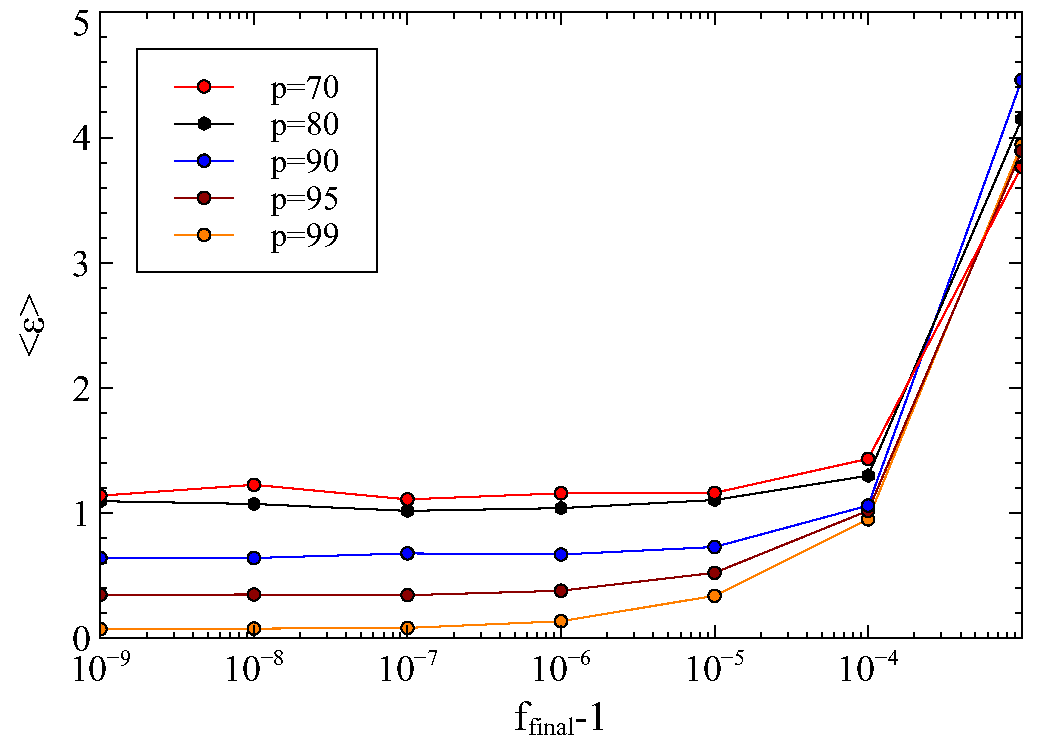
\includegraphics[scale=0.4, height=5cm]{wl_mean_error_f.pdf}
	\caption{Mean absolute error of the JDoS for the Ising model computed by the Wang-Landau sampling for a L4 SS lattice plotted against $f_{final}-1$. The values were averaged over $100$ simulations. }
	\label{error_abs_wl}
\end{figure}

	In originally proposed WL method, due to the biased samples at the initial stages of the computations, the final estimation of the JDoS will converge, with high precision, to a inaccurate solution independent of the flatness criteria and $f_{final}$ value used, shown in Figure \ref{error_abs_wl}. 

\begin{figure}[ht]
\centering
\subfigure[]{%
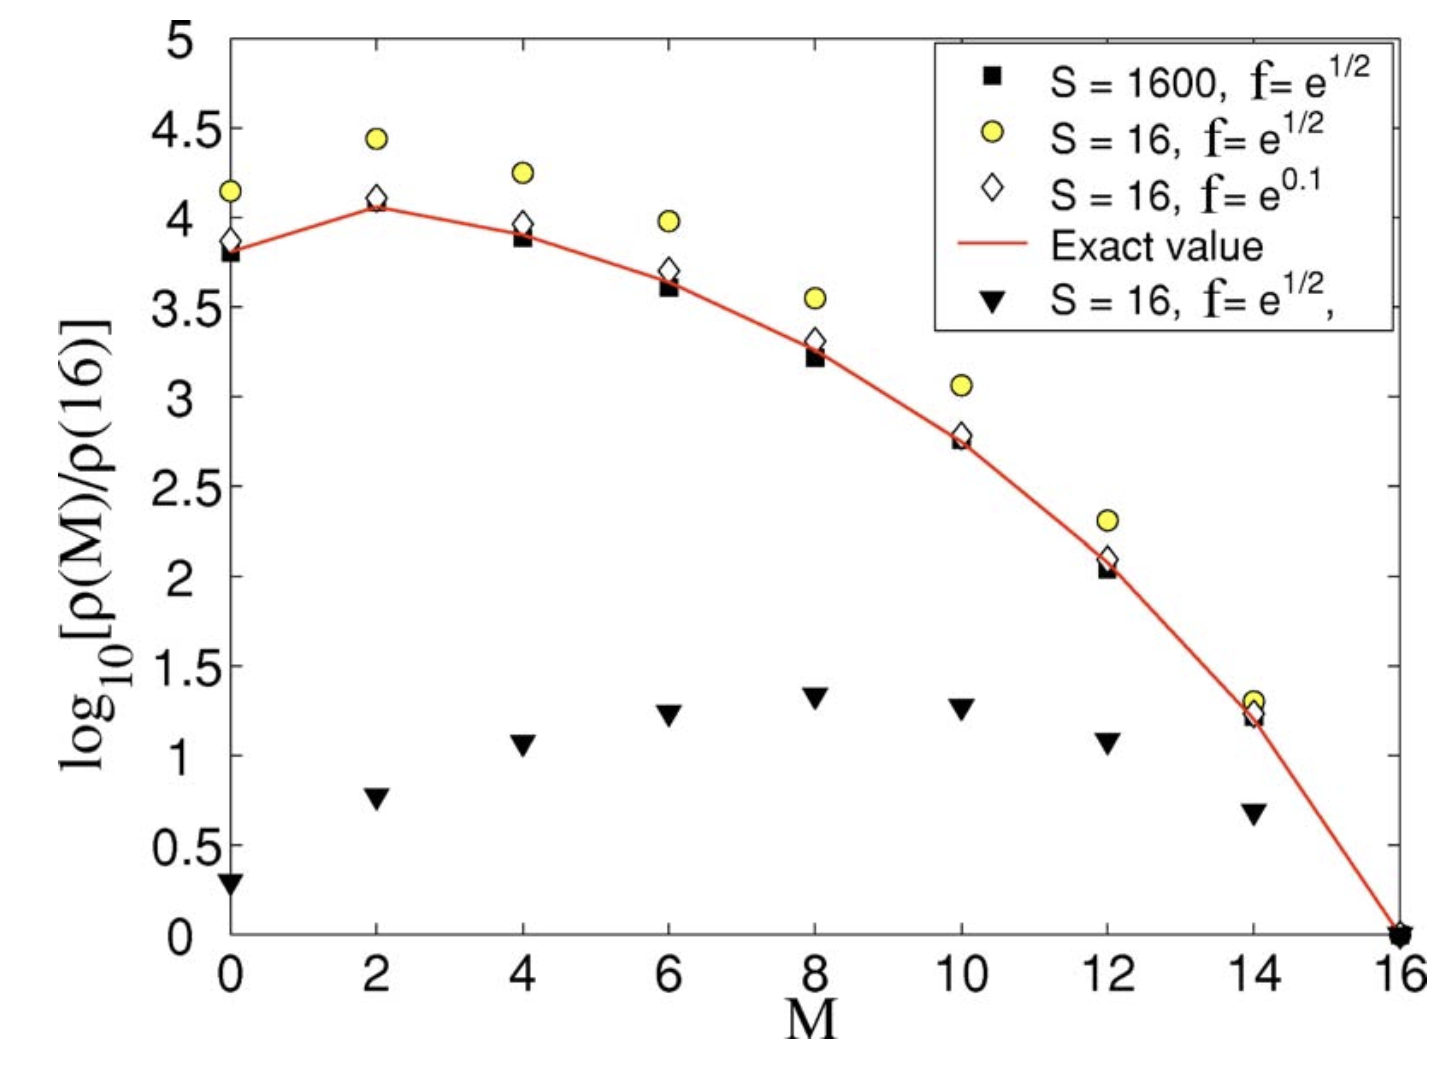
\includegraphics[scale=0.6, height=5cm]{S_paper_fig.png}
\label{S_parameter}}
\quad
\subfigure[]{%
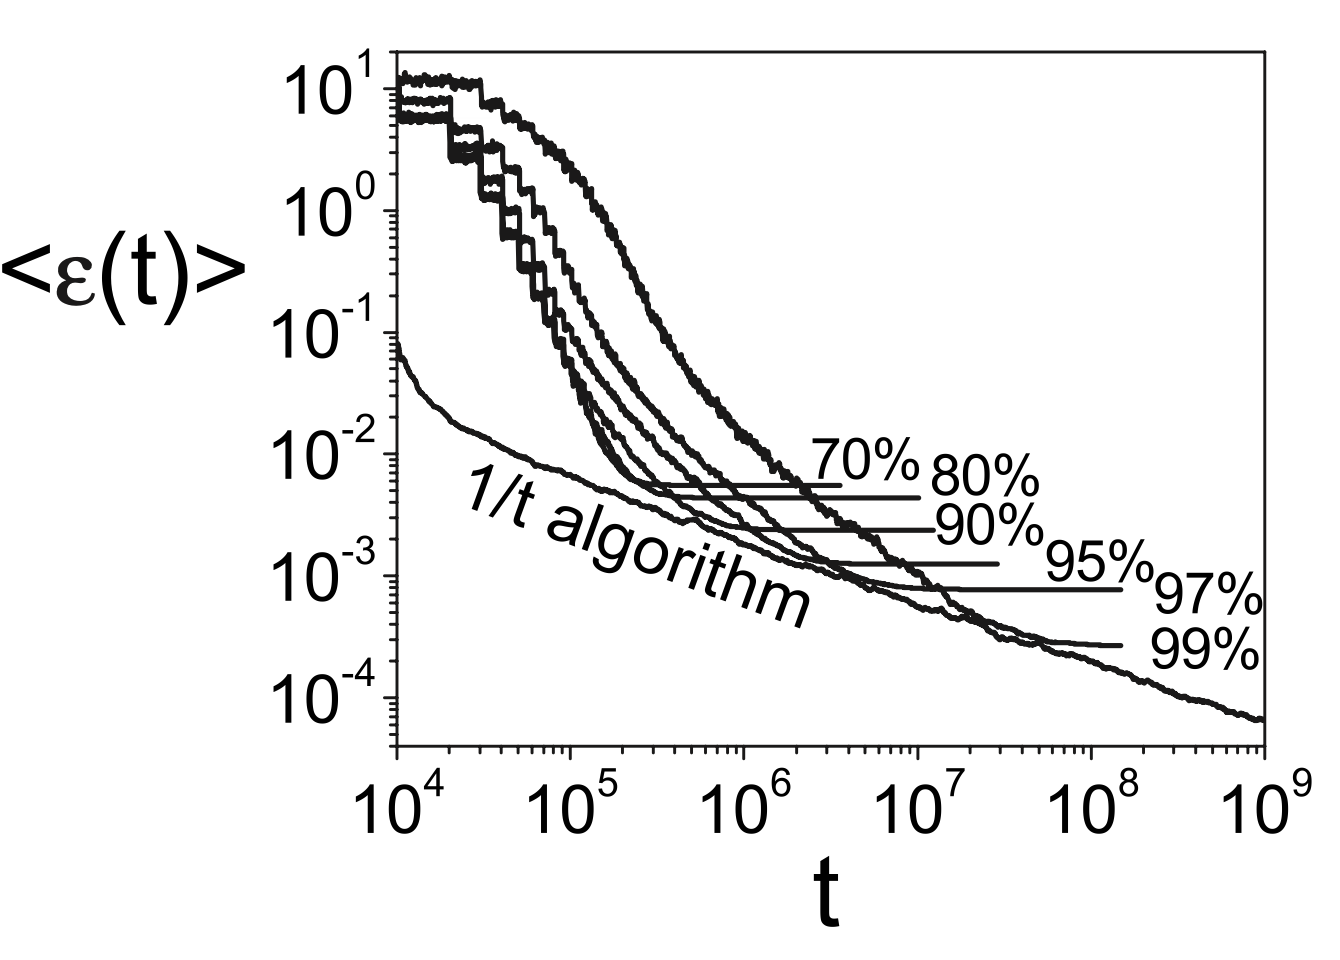
\includegraphics[scale=0.6, height=5cm]{t_paper_fig.png}
\label{t_algorithm}}

\caption{(a) $g(M)$, the density of states for magnetization $M$ of L4 SS Ising lattice normalized. The solid line connects the exact values, and the symbols were obtained with different parameters $f$ and $S$. Data was averaged over $100$ measurements, so the statistical errors are smaller than the symbols. Taken from \cite{Zhou2005}.  (b) Comparison between the mean error computed by the original WL for different flatness criteria and the mean error calculated using the $1/t$ time-dependent algorithm for a L8 SS Ising lattice. Taken from \cite{Belardinelli2007}.}

\end{figure}

%\begin{figure}[h]
%	\centering
%	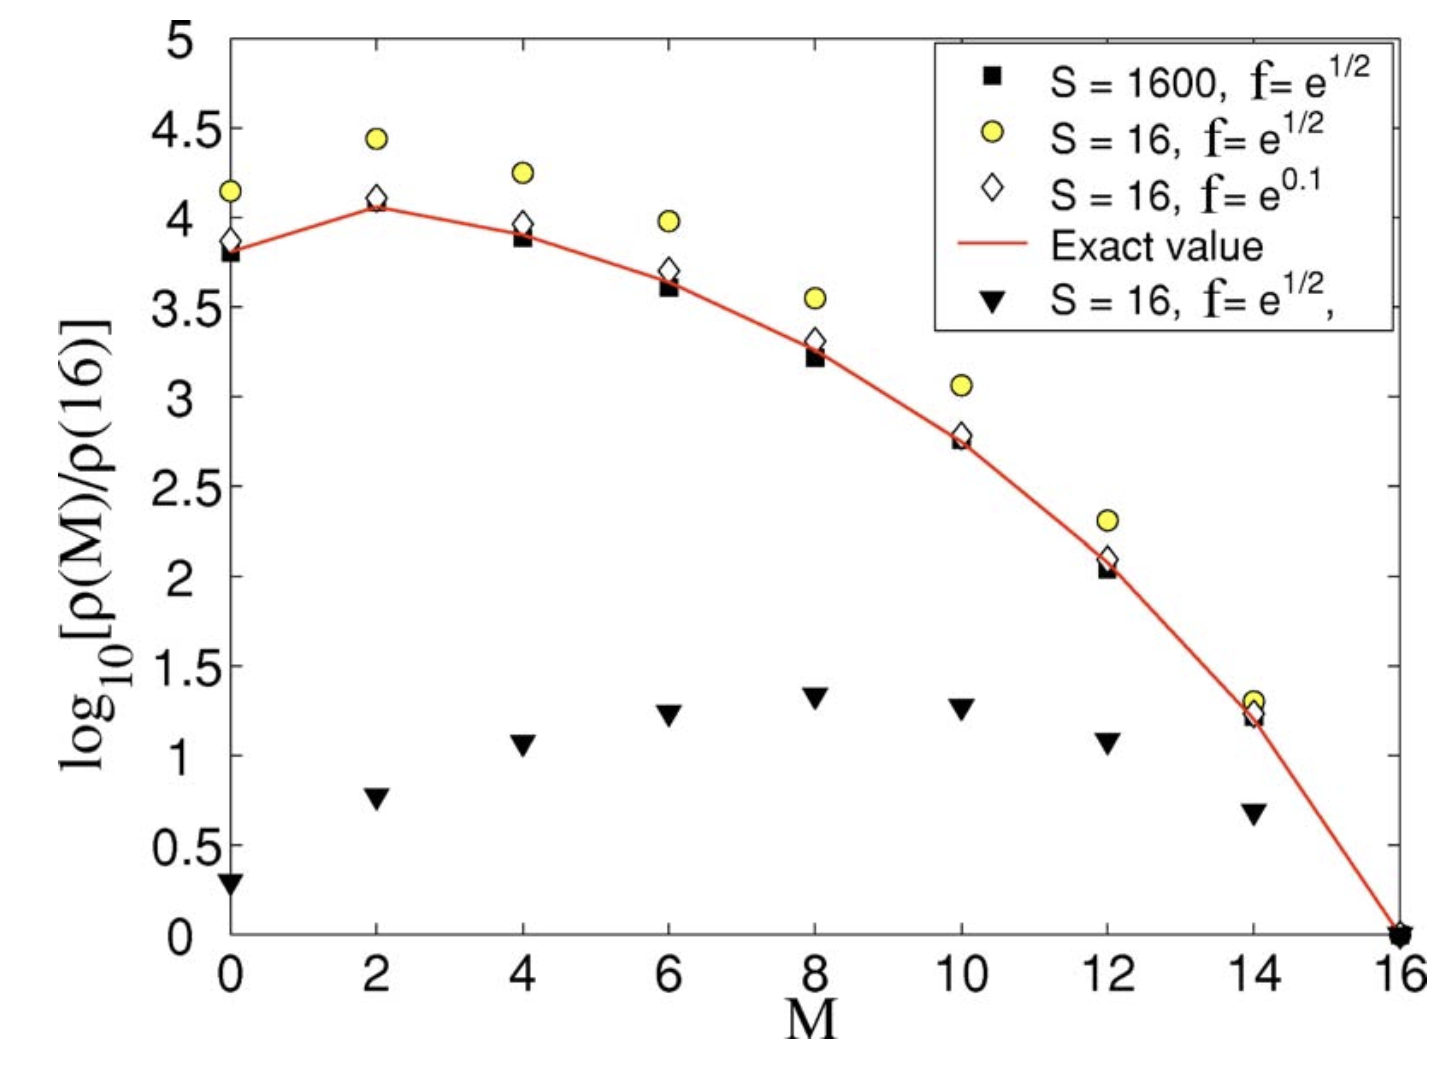
\includegraphics[scale=0.6, height=5.5cm]{S_paper_fig.png}
%	\caption{$g(M)$, the density of states for magnetization $M$ of L4 SS Ising lattice normalized. The solid line connects the exact values, and the symbols were obtained with different parameters $f$ and $S$. Data was averaged over $100$ measurements, so the statistical errors are smaller than the symbols. Taken from \cite{Zhou2005}.}
%	\label{S_parameter}
%\end{figure}



%\begin{figure}[h]
%	\centering
%	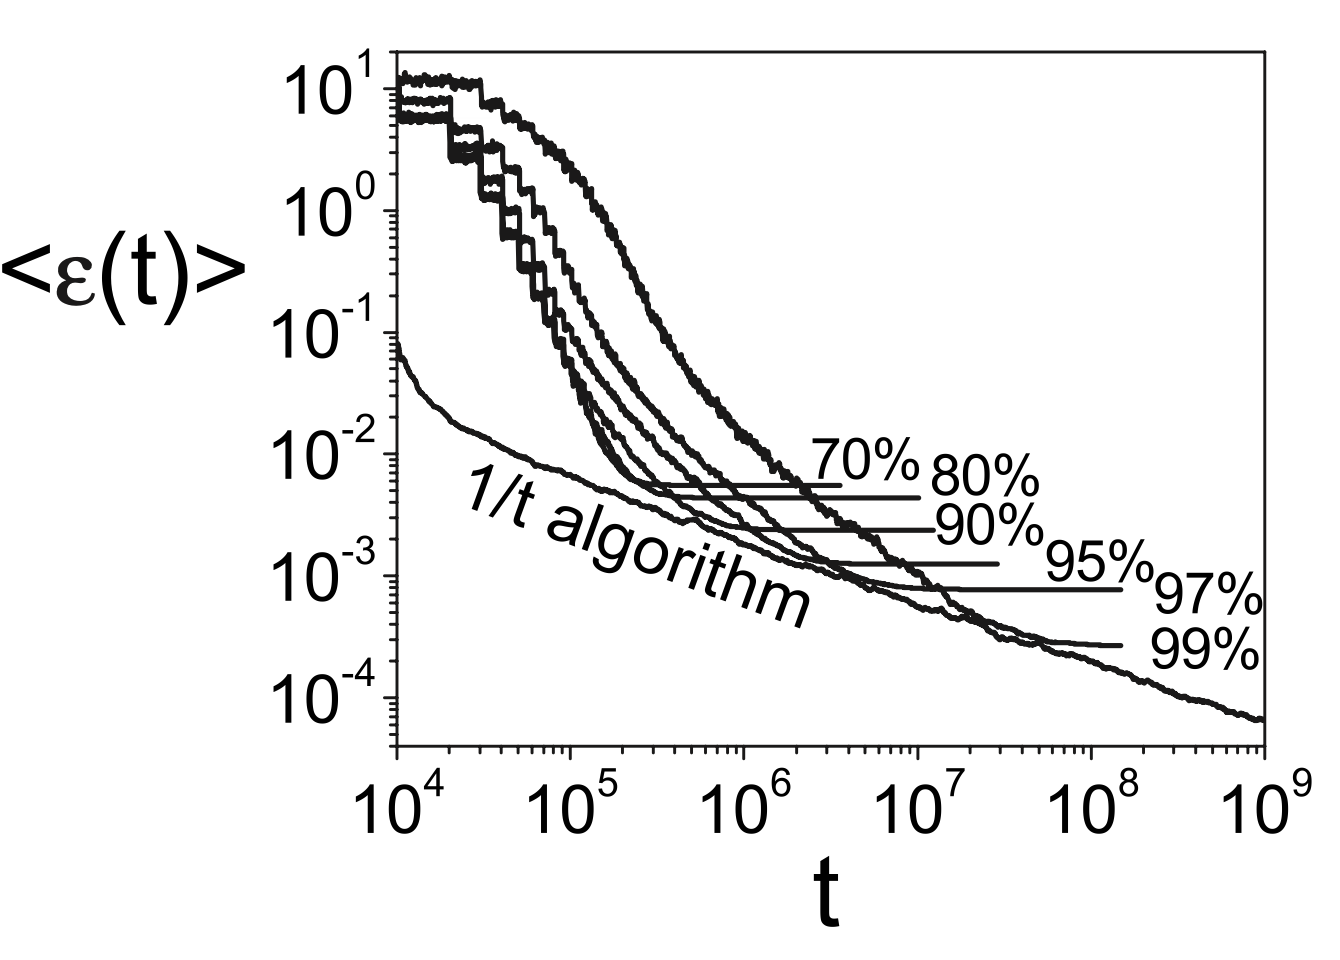
\includegraphics[scale=0.6, height=6cm]{t_paper_fig.png}
%	\caption{Comparison between the mean error computed by the original WL for different flatness criteria and the mean error calculated using the $1/t$ time-dependent algorithm for a L8 SS Ising lattice. Taken from \cite{Belardinelli2007}.}
%	\label{t_algorithm}
%\end{figure}

Either in its original forms, or using these more recent improvements, the WL method has become one of the go-to methods for DoS and JDoS estimation, because of its efficiency and ability to sample the whole phase space even if the estimation of the JDoS is not the most precise \cite{Zhou2005, Belardinelli2007}. It has been applied to magnetic systems like the Ising model, Lennard-Jones fluid simulations, biologic processes, etc \cite{Maerzke2014, Yan2002,Yan2003}.












